
\subsection{Теоретико-игровая интерпретация модели Барро-Гордона}

В игре участвуют два игрока: $p$ - правительство, $q$ - общественность, которые оперируют инфляцией $\pi$  и индексированием заработной платы $\omega$ соответственно. Для упрощения модели положим, что оба не могут прогнозировать будущие. Каждый игрок выбирает из следующих стратегий: низким $L$  и высоким  $H$ уровнем повышения. В общем виде игра может быть задана в виде матрицы выигрышей, 
\begin{table}[h]
	\centering
\begin{tabular}{|l|l|l|l|}
	\hline
	\multicolumn{2}{|l|}{\multirow{2}{*}{}} & \multicolumn{2}{l|}{Общественность} \\ \cline{3-4} 
	\multicolumn{2}{|l|}{}                  & $L$            & $H$            \\ \hline
	\multirow{2}{*}{Правительство}     & $L$     & $a,q$          & $b,v$          \\ \cline{2-4} 
	& $H$     & $c,x$          & $d,z$          \\ \hline
\end{tabular}
\end{table}\\
где параметры $a,b,c,d,q,v,x,z$  - выигрыши удовлетворяющие следующим ограничениям

\begin{equation}
c>a>d>b, q>v, q\ge z>x.
\label{eq:sec:ot:restrictions}
\end{equation}

В данном случае проще всего описать экономику через функцию совокупного предложения Лукаса

\begin{equation}
\label{eq:sec:ot:lucas}
y_t - Y = \lambda(\pi_t - \omega_t)+\varepsilon_t,
\end{equation}
где  $\lambda>0, y$  – производительность, $Y$ – естественный уровень производительности, а  $\varepsilon$ - макроэкономический шок близкий к нулю. Коэффициенты дисконтирования игроков составляют $\beta_g$ и $\beta_p$, а их функции  полезности  имеют следующий вид 

\begin{equation}
\label{eq:sec:ot:govUtil}
u^g_t=-(\pi_t - \tilde{\pi})^2 + \alpha y_t - \beta(y_t-Y)^2,
\end{equation}

\begin{equation}
\label{eq:sec:ot:pubUtil}
u^p_t=-(\pi_t - \omega)^2,
\end{equation}
где $\tilde{\pi}$ - оптимальный уровень инфляции, а $\alpha > 0, \beta > 0$ описывают относительный вес целей правительства (стабильной инфляции, высокой и стабильной производительности). Общественность озабочена верным ожиданием уровня инфляции для того, чтобы определить уровень зарплат на рынке. 
\\

Так как нас интересует эффект от выбранной политики, то сфокусируемся на долгосрочном исходе игры. Для этого однозначно определим экономику положив $\forall t$,      $\varepsilon_t=0$ , что подразумевает, что мы можем положить $\beta=0$ без потери общности. Из этого следует, что инструмент правительства $\pi$  представляет собой выбор средней инфляции.
\\

В стандартной пошаговой игре, в которой игроки могут менять свое поведение в каждый период, мы используем \eqref{eq:sec:ot:lucas}-\eqref{eq:sec:ot:govUtil} для получения равновесия

\begin{equation}
\label{eq:sec:ot:equilibrium}
\pi^*_t= \tilde{\pi} + \frac{\alpha\lambda}{2}= \omega^*_t,
\end{equation}
что является известным результатом $\pi^*_t > \tilde{\pi}$. Сфокусировав внимание на двух уровнях инфляции мы следуем ~\cite{ChoiAndMacui96InflationFinancialMarkets}, где были предложены два наиболее естественных варианта – оптимальный уровень из \eqref{eq:sec:ot:govUtil} и согласованного по времени из \eqref{eq:sec:ot:equilibrium}

\begin{equation}
\label{eq:sec:ot:optimal}
\pi \in \left\{L=\tilde{\pi}, H=\tilde{\pi}+\frac{\alpha\lambda}{2} \right\} \ni \omega^*_t.
\end{equation}

Мы можем, учитывая \eqref{eq:sec:ot:lucas}-\eqref{eq:sec:ot:pubUtil} и поделив на $\left(\frac{\alpha\lambda}{2}\right)$,  без потери общности вывести соответствующие выигрыши, представленные в таблице ниже. Так же вне зависимости от $\lambda$ и  $\alpha$ справедливы следующие ограничения для данной игры в дополнение к изначальным~(\ref{eq:sec:ot:restrictions})

\begin{equation}
	\label{eq:sec:ot:constraint}
	c>a=0 > d > b,c=-d=-\frac{b}{2}, q>v,q\ge z>x
\end{equation}

\begin{equation}
\label{eq:sec:ot:exampleConstraint}
c=1 > a=0 > d=-1 > b=-2, q=z=0 > v=x=-1,
\end{equation}

\begin{table}[h]
	\centering
	\begin{tabular}{|l|l|l|l|}
		\hline
		\multicolumn{2}{|l|}{\multirow{2}{*}{}} & \multicolumn{2}{l|}{Общественность} \\ \cline{3-4} 
		\multicolumn{2}{|l|}{}                  & $L$            & $H$            \\ \hline
		\multirow{2}{*}{Правительство}     & $L$     & $0,0$          & $-1,-1$          \\ \cline{2-4} 
		& $H$     & $\frac{1}{2},-1$          & $-\frac{1}{2},0$          \\ \hline
	\end{tabular}
	\caption{}	
	\label{table:sec:ot:real}
\end{table}


Стандартная пошаговая игра имеет уникальное равновесие по Нэшу $(H,H)$. Однако, оно неэффективно, так как является Парето доминированным. Это означает, что существует такой исход игры, который улучшит состояние одного, но при этом не ухудшит его для других игроков. В данном случае это «не Нэшовский» исход $(L,L)$.  У правительства возникает соблазн создать неожиданную инфляцию, чтобы повысить производительность и снизить уровень безработицы. Так как общественность рациональна, то будет ожидать высокую инфляцию – оба игрока будут в проигрыше. 


\subsection{Устойчивость равновесных стратегий в модели Барро-Гордона на
	временных шкалах} 

Рассмотрим игровую интерпретацию модели Барро-Гордона на временных шкалах.

Все допущения выдвинутые в стандартной игре остаются. Расширим их:
\begin{itemize}
	\item игра начинается одновременным ходом, 
	\item заранее известно неизменное количество ходов $r^g \in \mathbb{N}$ и $r^p \in \mathbb{N}$,
	\item игра заканчивается через $T$ периодов, где $T$ - наименьшее общее кратное для $r^g$ и $r^p$,
	\item игроки рациональны, обладают равноценными знаниями и полной информацией о структуре игры, матрице выигрышей и всех предыдущих ходах.
\end{itemize}

Другими словами определяется три временных шкалы: правительства, общественности и самой игры:
\begin{equation}
\label{eq:sec:tech:scales}
T_g = \{0,r^g,2r^g,...,T\}, T_p=\{0,r^p,2r^p,...,T\}, T=T_g\cup T_p 
\end{equation}

Главным преимуществом использования однородных временных шкал является экономическая интерпретация: $r^g$ и $r^p$ представляют собой степень возможности изменений политики относительно инфляции и степень реагирования для внесения изменений в заработные платы.
\\

Асинхронная игра на временных шкалах будет как правило иметь несколько равновесий по Нэшу, среди которых мы выберем лучшую в зависимости от под-игры.

\begin{theorem}
	Рассмотрим общую несогласованную по времени игру на однородных временных шкалах, для которой выполняются~(\ref{eq:sec:ot:constraint}) и ~(\ref{eq:sec:tech:scales}). Тогда все SNPE игры будут SNPE Рамсея, если и только если
	
	\begin{equation}
	\label{eq:sec:tech:theoremSystem}
	r^g> \bar{r^g}(R) = \left\{ 
	\begin{aligned} 
	&\frac{c - d}{a-d}r^p= \frac{a-b}{a-d}r^p, &&\text{если } R=0
	\\
	&\frac{(1+R)(c-d)}{a-d}r^p= \frac{a-b + R(c-d)}{a-d}r^p, &&\text{если } 	R\in(0; \bar{R})
	\\
	&\frac{c-d-(1-R)(a-b)}{a-d}r^p= \frac{(a-b)}{a-d}Rr^p, &&\text{если } 	R\in(\bar{R};1)
	\end{aligned}
	\right.		
	\end{equation}
\end{theorem}
где $\bar{R}=\frac{q-v}{z-x+q-v}$. В несогласованной игре, где справедливо ~(\ref{eq:sec:ot:constraint}),  ~(\ref{eq:sec:tech:theoremSystem}) преобразуется в 

\begin{equation}
\frac{r^g}{r^p} \in \left(\frac{3}{2}, 2\right)\cup \left(\frac{5}{2}, \infty\right)
\end{equation}
Доказательство: смотреть Либиха и Штелиха ~\cite{libichIncorpo}.


Можно утверждать, что действия игроков могут не всегда быть детерминистическими и/или что частота их ходов различается во времени или подчиняется некоторому случайному процессу. Разнородные временные шкалы позволяют изучать подобные случаи. Для большей эффективности нормализуем горизонт планирования как $T = r^g$. Как и ранее игроки $g$ и $p$ ходят одновременно в первом периоде и во всех $T = r^g$ периодах, в промежутках между которыми общественность так же способна реагировать на ход правительства. Для удобства сравнения оставим все предположения предыдущего параграфа неизменными.

Рассмотрим произвольную временную шкалу $\mathbb{T}$ и произвольную невозрастающую функцию реакции общественности $f : \mathbb{T} \to [0,1]$. В данной работе рассматриваются два представляющих интерес особых случая. В первом, при разнородной (атомистической) общественности, функция реакции может быть интерпретирована как часть общественности, которая уже имела возможность совершить ход. Во втором, при вероятностных ходах общественности, функция реакции может быть интерпретирована как кумулятивная функция распределения её ходов.

Чтобы удостовериться в том, что все SPNE являются SPNE Рамсея, достаточно показать, что в первом ходе оптимальной стратегией $g$ является $L$ вне зависимости от хода общественности в первом периоде. Получим два соответствующих условия:
\begin{equation}
\label{sec:hetero:main1}
ar^g > c \int_0^{r^g} 1 - f(t) \Delta t + d  \int_0^{r^g} f(t) \Delta t ,
\end{equation}
\begin{equation}
\label{sec:hetero:main2}
dr^g > b \int_0^{r^g} 1 - f(t) \Delta t + a  \int_0^{r^g} f(t) \Delta t .
\end{equation}

\begin{theorem}
	\label{spneTh}
	Рассмотрим общую несогласованную по времени игру, в которой выполняется~\eqref{eq:sec:ot:constraint} и $f : \mathbb{T} \to [0,1]$ -- невозрастающая функция реакции. Тогда все SPNE игры являются SPNE Рамсея тогда и только тогда, когда выполняется неравенство
	\begin{equation}
	\label{sec:hetero:main3}
	\int_0^{r^g} f(t) \Delta t > \frac{r^g}{2} .
	\end{equation}
\end{theorem}

Для лучшей наглядности теоремы~\ref{spneTh} и лучшего понимания приведём несколько следствий и рассмотрим пример. Как уже было указано ранее, мы концентрируемся на двух случаях: разнородной общественности и вероятностных моделях.

\subsubsection{Разнородная общественность.} Во-первых, предположим, что существует $N$ различных общественных групп (профсоюзов) $p_1,...,p_N$ с соответствующими $r^{p_1},...,r^{p_N}$ и размерами $s_1,...,s_N \in [0,1]$, которые удовлетворяют естественному предположению $\sum_{i=1}{N}s_i = 1$. Чтобы свести наше внимание к первому ходу правительства, предположим что $r^g$ является кратным для $r^{p_i}$ для всех $i = 1,...,N$, то есть
$$ \frac{r^g}{r^{p_i}} \in \mathbb{N}.$$
Для более асинхронных случаев  см.~\cite{libichIncorpo}. Для данного особого случая теорему~\ref{spneTh} можно переписать следующим образом.\\
\textbf{Следствие 1.} \textit{Рассмотрим общую несогласованную по времени игру, в которой выполняется~\eqref{eq:sec:ot:constraint} и общественность состоит из $N$ различных групп. Тогда все SPNE игры являются SPNE Рамсея тогда и только тогда, когда выполняется неравенство
	\begin{equation}
	\label{sec:hetero:main4}
	\sum_{i=1}^N s_i(r^g - r^{p_i}) \geq \frac{r^g}{2} .
	\end{equation}
}
%опять же доказательство

\subsubsection{Вероятностная модель.}
Вернёмся к случаю с унифицированной общественностью, чтобы рассмотреть вероятностные ходы отдельно от влияния эффектов разнородной общественности. В зависимости от результатов переговоров общественность будет реагировать на первый ход правительства в какой-то момент времени из интервала $[a,b], 0< a < b < r^g$, с равномерно распределённым вероятностным законом. Теорема~\ref{spneTh} принимает вид:\\
\textbf{Следствие 2.} \textit{Рассмотрим общую несогласованную по времени игру, в которой выполняется~\eqref{eq:sec:ot:constraint} и общественность делает второй ход в какой-то момент времени из интервала $[a,b]$ с равномерно распределённым вероятностным законом. Тогда все SPNE игры являются SPNE Рамсея тогда и только тогда, когда выполняется неравенство
	\begin{equation}
	\label{sec:hetero:main5}
	\frac{b^2 - a^2}{2} \geq b - \frac{r^g}{2} .
	\end{equation}
}
Очевидно, что можно рассматривать произвольные комбинации описанных выше подходов, то есть разнородных игроков с вероятностными ходами, вероятность которых может быть описана некоторыми функциями распределения. Приведём пример.\\
\textbf{Пример 1.} Рассмотрим экономику с двумя профсоюзами, каждый их которых состоит из $s_1$ и $s_2$ рабочих соответственно, так что выполняется $s_1 + s_2 = 1$. Примем в качестве одного периода квартал (раз в квартал выпускаются сводки по макроэкономике). Предположим, что $r^g = 5$ и что время реакции профсоюзов составляют как минимум  1 и 3 квартала, но как максимум -- 1,5 и 3,5 квартала соответственно. Для простоты предположим, что решение, принятое за полтора квартала подчиняется равномерному закону распределения. Тогда получим:
$$ \mathbb{T} :={0} \cup [1, 1.5] \cup {r^g} ,$$
$$ \mathbb{T} :={0} \cup [3, 3.5] \cup {r^g} .$$
Функция реакции тогда имеет вид $f : \mathbb{T}_1\cup\mathbb{T}_2\to[0,1]$:
$$ f(x)\left\{  
\begin{array}{l c l}
0 & if & x = 0,\\
2s_1(x - 1) & if & x \in [1,1.5],\\
s_1 + 2s_2(x - 3) & if & x \in [3,3.5],\\
1 & if & x = 5.
\end{array} 
\right.$$
Интегрируя по $\mathbb{T}_1\cup\mathbb{T}_2$ получим
$$ \int_0^5 f(x) \Delta x = \frac{15}{4}s_1 + \frac{7}{4}s_2. $$
Предположение~\eqref{sec:hetero:main3} теоремы~\ref{spneTh} удовлетворяется (и следовательно единственное равновесие является равновесием Рамсея) тогда и только тогда, когда выполняется
$$ s_1 \geq \frac{3}{8}, \text{или, что эквивалентно,} s_2 \leq \frac{5}{8}. $$
Интуитивно понятно, что профсоюз, принимающий решения быстрее, должен быть достаточно велик для того, чтобы общая реакция общественности была достаточно быстрой, чтобы препятствовать увеличению инфляции правительством.

\subsection{Классическая модель профсоюз---монополист}
\label{sec:monopoly}

Данная модель является моделью отношений профсоюз-фирма по Леонтьеву~\cite{LeontiefW}, в которой профсоюз задаёт уровень заработной платы, после чего фирма выбирает желаемое количество наёмных работников (уровень найма). Предположим что фирма оперирует в условиях конкурентного рынка с рыночной ценой $P$.\\

Порядок игры следующий:\\
\textbf{Первый этап.} Профсоюз устанавливает уровень заработной платы $W$.\\
\textbf{Второй этап.} Фирма выбирает уровень найма $E$.\\

Выигрыши составляют:\\
Функция полезности профсоюза имеет вид 
$$ U = U(W,E), \quad \frac{\partial U}{\partial W} > 0; \quad \frac{\partial U}{\partial E}~>~0.$$ 
Например $U = \lambda WE.$, где $\lambda \in (0; 1)$\\
Полезность для фирмы измеряется как прибыль 
$$\Pi~=~PY(\bar K,E)~-~WE,$$ 
где цена $P$ дана, а капитал $\bar K$ фиксирован. Отсюда мы можем переписать 
$$\Pi(W,E)~=~R(E)~-~WE,$$ 
где $R$ -- доход.\\

Решение методом обратной индукции:\\
\textbf{Второй этап.} Фирма максимизирует свою прибыль по $E$ при заданном уровне заработной платы. Условие первого порядка примет вид
$$ W = R'(E) = MPE. $$
Разрешая относительно $E$ получим кривую спроса: $E~=~g(W)$.\\
\textbf{Первый этап.} Решается
$$ \max_W U(W,E) = U(W,g(W)). $$
Решение приведено на графике~\ref{fig:monopoly_union}. Графически можно показать, что исход игры неэффективен. Точка $X$ является точкой равновесия обратной индукции модели монополии профсоюза. Точки в закрашенной области Парето-предпочтительнее $X$. $AB$ является кривой контракта, состоящей из точек, в которых изо-профиты и кривые безразличия профсоюза имеют общий тангенс~\cite{ShandongUniver}.


\begin{figure}[h]
	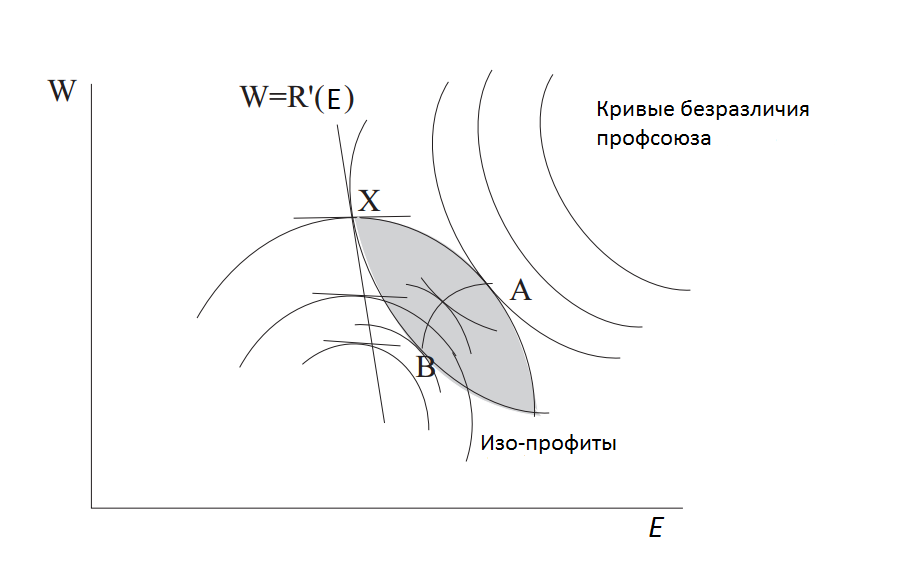
\includegraphics[width=1.0\linewidth]{monopoly_union.png}
	\caption{}
	\label{fig:monopoly_union}
\end{figure}

\subsection{Модель профсоюз---монополист на временных шкалах}

В игре, как и в непрерывной модели присутствует два игрока: профсоюз $P$ и фирма $F$, чьими рычагами влияния на игру являются $W$ - зарплата рабочего и $E$ - количество нанятых рабочих соответственно.
Каждый игрок выбирает из следующих стратегий: низким $L$ и высоким $H$ уровнем повышения. В общем виде игра может быть задана следующей матрицей выигрышей: 

\begin{table}[h]
	\centering
	\begin{tabular}{|l|l|l|l|}
		\hline
		\multicolumn{2}{|l|}{\multirow{2}{*}{}} & \multicolumn{2}{l|}{Профсоюз} \\ \cline{3-4} 
		\multicolumn{2}{|l|}{}                  & $L$            & $H$            \\ \hline
		\multirow{2}{*}{Фирма}     & $L$     & $a,q$          & $b,v$          \\ \cline{2-4} 
		& $H$     & $c,x$          & $d,z$          \\ \hline
	\end{tabular}
\end{table}
Функция полезности профсоюза  $U_t(W,E)=\lambda WE$, где $\lambda \in(0;1)$:
$$\frac{\partial U}{\partial W} > 0; \quad \frac{\partial U}{\partial E}~>~0 \quad U(0,E)=U(W,0)=U(0,0)=0,$$


Функция полезности фирмы $\Pi_t(W,E)=cP(\bar{K},E)-WE$:
$$P(\bar{K}, E)=A\bar{K}^\alpha E^\beta,$$ где $A$ – коэффициент нейтрального технического прогресса, $\alpha$ и $\beta$ – коэффициенты эластичности валового внутреннего продукта по капитальным и трудовым затратам.\\

Для профсюза соотношения функции полезности для всех стратегий будет следующим:
\begin{equation}
U(L,L) < U(L,H) \thickapprox U(H, L) < U(H,H),
\end{equation}
где соотношение $U(L,H) \thickapprox U(H, L)$ неопределенное, так как это чисто "политический" момент, что для профсоюза более выгодно: большее количество людей, получающих меньшую зарплату или меньшее количество людей, получающих большую зарплату. 

Для нахождения соотношений между функциями полезности для фирмы построим график~\ref{fig:monopoly_union1}.

\begin{figure}[h]
	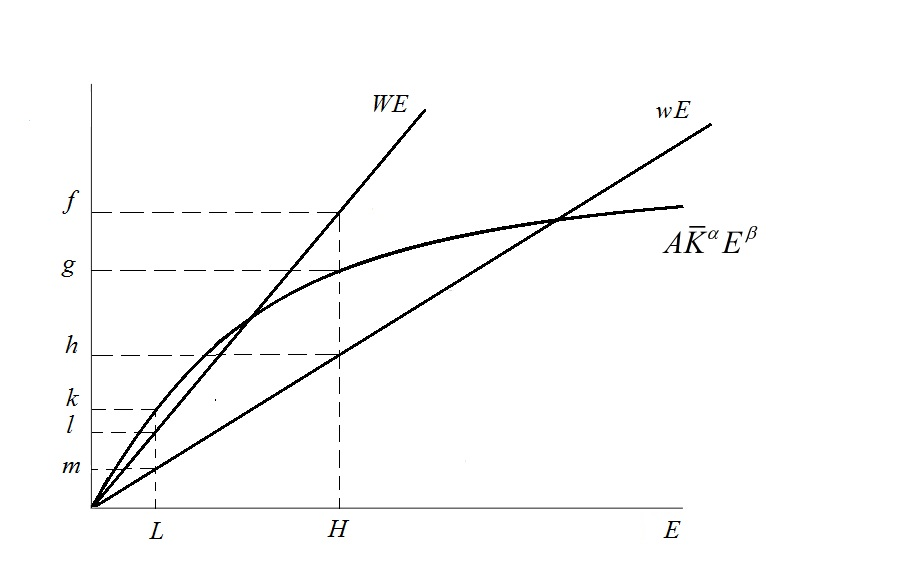
\includegraphics[width=1.0\linewidth]{monopoly_union2.jpg}
	\caption{}
	\label{fig:monopoly_union1}
\end{figure}

где $w$ - низкий уровень зарплат по стратегии $L$, а $W$ - высокий уровень зарплат по стратегии $H$. 
Принимая во внимание, что все коэффициенты константы за исключением количества нанятых и уровня зарплат, легко вывести следующее:

\begin{equation}
\Pi(H,H)=g-f < \Pi(H,L)=k-l < \Pi(L, L)=k-m < \Pi(L,H)=g-h.
\end{equation}
Следовательно матрица выигрышей будет следующей:
\begin{table}[h]
	
	\centering
	\begin{tabular}{|l|l|l|l|}
		\hline
		\multicolumn{2}{|l|}{\multirow{2}{*}{}} & \multicolumn{2}{l|}{Профсоюз} \\ \cline{3-4} 
		\multicolumn{2}{|l|}{}                  & $L$            & $H$            \\ \hline
		\multirow{2}{*}{Фирма}     & $L$     & $a,q$          & $b,v$          \\ \cline{2-4} 
		& $H$     & $c,x$          & $d,z$          \\ \hline
	\end{tabular}
	\caption{}
	\label{table:firm}
	
	
\end{table}\\
где $q < x \thickapprox v < z, 0 > d < b < a < c$
